\documentclass[10pt,a4paper]{article}
\usepackage[T1]{fontenc}
\usepackage[utf8]{inputenc}
\usepackage[scaled=0.95]{helvet}
\renewcommand{\familydefault}{\sfdefault}
\usepackage[a4paper,left=17mm,right=17mm,top=20mm,bottom=20mm]{geometry}
\usepackage{amsmath}
\usepackage{graphicx}
\usepackage{booktabs}
\usepackage{tabularx}
\usepackage{xcolor}
\usepackage{enumitem}
\usepackage{fancyhdr}
\usepackage{lastpage}
\usepackage{titlesec}
\usepackage{tcolorbox}
\usepackage{caption}
\usepackage{needspace}
\usepackage[hidelinks]{hyperref}

\definecolor{navy}{HTML}{1F3864}
\definecolor{ink2}{HTML}{52514E}
\definecolor{rule}{HTML}{BFBFBF}
\definecolor{tint}{HTML}{EEF3FA}

\setlength{\parindent}{0pt}
\setlength{\parskip}{5pt}
\setlist{nosep,leftmargin=12pt}
\titleformat{\section}{\color{navy}\large\bfseries}{\thesection}{6pt}{}
\titleformat{\subsection}{\color{navy}\normalsize\bfseries}{\thesubsection}{6pt}{}
\titlespacing*{\section}{0pt}{10pt}{3pt}
\titlespacing*{\subsection}{0pt}{7pt}{2pt}
\renewcommand{\arraystretch}{1.12}

\pagestyle{fancy}
\fancyhf{}
\renewcommand{\headrulewidth}{0.4pt}
\fancyhead[L]{\small\color{ink2}Bouvet ASA (BOUV NO) \textbar{} Equity research}
\fancyhead[R]{\small\color{ink2}12 February 2026}
\fancyfoot[L]{\footnotesize\color{ink2}Student case analysis. Not investment advice. See disclaimer on the last page.}
\fancyfoot[R]{\footnotesize\color{ink2}Page \thepage\ of \pageref{LastPage}}

\newcolumntype{R}{>{\raggedleft\arraybackslash}X}

\begin{document}

{\color{navy}\Large\bfseries Bouvet: trough earnings are priced, the 2027 recovery is not}\par
\vspace{2pt}
{\color{ink2}IT consultancy, Norway \textbar{} Forvaltningsgruppen at TIHLDE \textbar{} Pareto Securities Equity Research Case 2026}

\vspace{4pt}
\begin{minipage}[t]{0.63\textwidth}
\vspace{0pt}
\setlength{\parskip}{5pt}
Bouvet's 2025 slowdown came from utilisation, not lost clients. The billing ratio fell 1.6, 1.7 and 2.1 percentage points year on year in Q1, Q2 and Q3 2025, while headcount held at about 2,350 FTE and 97\% of revenue still came from existing customers. Pricing has lost its edge: hourly price growth slowed to 2.9\% in Q3'25, roughly the pace of realised personnel cost per FTE (2.7\% in 9M'25) and below the 4.2\% wage settlement. We therefore model a flat 2026, with EBITDA margin at 14.8\% against 14.9\% in 2025E, and recovery to 16.1\% in 2027E as utilisation normalises and the calendar adds two working days.

At NOK 54.7 the shares trade on 14.5x our 2026E EPS, against an average of about 19x trailing over 2023 to 2025. The market is extrapolating the trough. A mid-year DCF at a 9.0\% cost of equity gives NOK 73.9 and peer multiples with a 30\% premium give NOK 60.9. The 50/50 blend is NOK 67.4 today, which rolls to a 12-month target of \textbf{NOK 70}. With a 6.5\% dividend yield the expected total return is +34.5\%, more than 5 percentage points above the cost of equity, so we rate the shares \textbf{BUY}.

\textbf{What would change our view.} A fourth quarter of falling billing ratio, or a 2026 wage settlement well above 4\%, puts us in the bear case (target NOK 44, $-$13\% total return).
\end{minipage}\hfill
\begin{minipage}[t]{0.34\textwidth}
\vspace{0pt}
\begin{tcolorbox}[colback=tint,colframe=navy,boxrule=0.6pt,arc=1pt,left=5pt,right=5pt,top=4pt,bottom=4pt]
{\color{navy}\Large\bfseries BUY}\hfill{\color{navy}\bfseries TP NOK 70}\par
\vspace{2pt}
\small
\begin{tabularx}{\linewidth}{@{}Xr@{}}
Share price (NOK) & 54.7 \\
Upside to target & +28.0\% \\
Dividend yield (next 12m) & 6.5\% \\
Expected total return & +34.5\% \\
Cost of equity & 9.0\% \\
\midrule
Market cap (NOKm) & 5,678 \\
Shares (m) & 103.8 \\
Cash ex leases, Q3'25 & 373 \\
Cash ex leases, 31 Dec 2025E & 435 \\
Lease liabilities, Q3'25 & 353 \\
NIBD incl. leases & $-$20.9 \\
\midrule
Bear / Bull target & 44 / 90 \\
Top 10 customers & 68\% \\
Oil \& gas / power / public & 42 / 20 / 18\% \\
\end{tabularx}
\end{tcolorbox}
\end{minipage}

\vspace{2pt}
\begin{center}
\small
\begin{tabularx}{\textwidth}{@{}lRRRRR@{}}
\toprule
\textbf{Base case} & \textbf{2024A} & \textbf{2025E} & \textbf{2026E} & \textbf{2027E} & \textbf{2028E} \\
\midrule
\textbf{Revenue (NOKm)} & \textbf{3,921} & \textbf{3,934} & \textbf{4,069} & \textbf{4,352} & \textbf{4,581} \\
\quad growth & 11.2\% & 0.3\% & 3.4\% & 7.0\% & 5.3\% \\
EBITDA (NOKm) & 611 & 586 & 604 & 699 & 727 \\
\quad margin & 15.6\% & 14.9\% & 14.8\% & 16.1\% & 15.9\% \\
EBIT (NOKm) & 490 & 488 & 502 & 591 & 613 \\
\quad margin & 12.5\% & 12.4\% & 12.3\% & 13.6\% & 13.4\% \\
\textbf{EPS (NOK)} & \textbf{3.71} & \textbf{3.64} & \textbf{3.77} & \textbf{4.43} & \textbf{4.60} \\
DPS (NOK) & 3.62 & 3.55 & 3.68 & 4.33 & 4.49 \\
P/E at NOK 54.7 & 14.7x & 15.0x & 14.5x & 12.3x & 11.9x \\
EV/EBIT (IFRS 16) & 11.5x & 11.6x & 11.3x & 9.6x & 9.2x \\
Dividend yield & 6.6\% & 6.5\% & 6.7\% & 7.9\% & 8.2\% \\
Average FTE & 2,345 & 2,350 & 2,362 & 2,409 & 2,469 \\
Working days & 250 & 250 & 251 & 253 & 251 \\
\bottomrule
\end{tabularx}
\end{center}
{\footnotesize\color{ink2}Source: Bouvet quarterly reports (Model tab), case model. 2025E is 9M'25 reported plus our Q4'25 estimate. EV uses NIBD including lease debt, consistent with IFRS 16 EBIT.}

\begin{center}
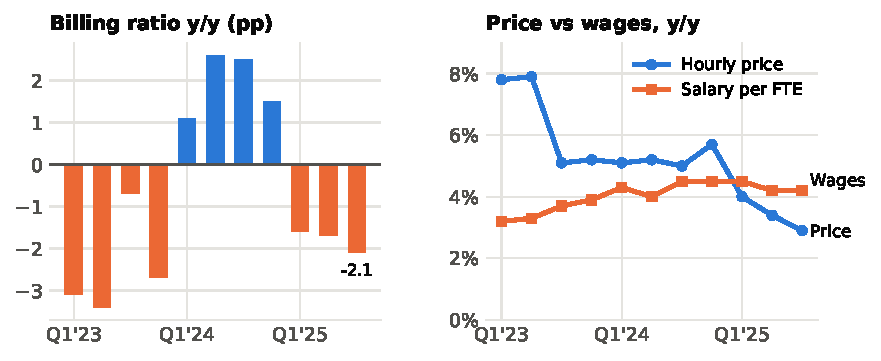
\includegraphics[width=0.86\textwidth]{figures/fig_kpi.pdf}
\vspace{-6pt}
\captionof*{figure}{\footnotesize\color{ink2}Left: utilisation turned negative again in 2025. Right: price growth fell below the wage settlement from Q1'25; realised cost per FTE grew less (2.7\% in 9M'25). Source: Bouvet quarterly reports.}
\end{center}

\newpage
\needspace{12\baselineskip}
\section{Company overview}
Bouvet sells consultant hours. About 2,350 FTE across Norwegian regional offices and a small Swedish unit bill clients by the hour, so revenue is the product of three things we can forecast separately:
\begin{gather*}
\text{Revenue}_t = \overline{\text{FTE}}_t \times \text{Working days}_t \times \text{Revenue per FTE-day}_t \\
\text{Revenue per FTE-day}_t = \text{Revenue per FTE-day}_{t-1}\,(1+g^{\text{price}}_t)\,(1+g^{\text{utilisation}}_t)
\end{gather*}
Salaries are the dominant cost and are paid per FTE, not per billable day. That makes earnings sensitive to anything that moves revenue per FTE: a 1\% change in 2026E revenue per FTE-day moves EBITDA by about 6\%. The same logic explains why the calendar matters. Working days in the model come from \texttt{NETWORKDAYS} on a Norwegian holiday table, which reproduces Bouvet's reported working days exactly for every year from 2021 to 2024 and for each reported quarter of 2025 (Q1 to Q3).

The client base is concentrated and sticky. Existing customers made up 97\% of revenue in Q3'25 and the top 10 customers 68\%. Oil and gas is the largest end market at 42\%, followed by power supply at 20\% and public administration at 18\%.

\needspace{12\baselineskip}
\section{Market overview}
The submission sized Norwegian IT services at USD 8.2bn in 2024, with IT consulting and systems integration at USD 4 to 5bn and 5.2\% annual growth to 2028 (Statista and Mordor Intelligence, as cited in the case deck; we have not re-verified these figures). Bouvet's NOK 3.9bn of revenue is roughly 4.5\% of that market. The more useful evidence for 2026 is how peers are trading through the downturn:

\begin{center}
\small
\begin{tabularx}{0.9\textwidth}{@{}lRRRRR@{}}
\toprule
\textbf{Revenue, NOKm} & \textbf{Q4'24} & \textbf{Q1'25} & \textbf{Q2'25} & \textbf{Q3'25} & \textbf{QoQ trend} \\
\midrule
Bouvet & 1,026 & 1,075 & 969 & 870 & $-$5.1\% \\
Knowit & 1,642 & 1,594 & 1,491 & 1,222 & $-$9.1\% \\
Webstep & 255 & 236 & 215 & 178 & $-$11.2\% \\
Itera & 212 & 232 & 202 & 173 & $-$6.0\% \\
\bottomrule
\end{tabularx}
\end{center}
{\footnotesize\color{ink2}Source: company reports as compiled in the case workbook (Peer table). Q3 is seasonally weak for all four.}

Bouvet is losing less than its listed Nordic peers. Our variant view is that this resilience, together with a net cash balance sheet and a payout ratio near 100\%, is not reflected in a share price that sits inside our bear-to-base multiples range (NOK 48 to 60.9).

\needspace{12\baselineskip}
\section{Financials and estimates}
\needspace{8\baselineskip}
\subsection{Forecast method}
Historical years pull from the reported data with \texttt{INDEX}/\texttt{MATCH}. 2025E adds a Q4'25 estimate to nine months of actuals: Q4'24 revenue per FTE-day, adjusted for the Q3'25 year-on-year change, times Q3'25 closing FTE and 62 working days. From 2026E every driver is set by scenario, and a single selector on the Inputs sheet switches the whole model with \texttt{INDEX}. Drivers fade linearly to long-run values by 2035E; in the long run price and wage growth are equal, so margins are stable. Subcontractor cost and other opex stay at their 2025E share of revenue. Subcontracting has fallen every year since 2022, so a multi-year average would overstate cost.

\begin{center}
\small
\begin{tabularx}{\textwidth}{@{}llRRRR@{}}
\toprule
\textbf{Driver} & \textbf{Scenario} & \textbf{2026E} & \textbf{2027E} & \textbf{2028E} & \textbf{Long run} \\
\midrule
FTE growth & Bear & $-$3.0\% & 0.0\% & 1.0\% & 0.0\% \\
 & Base & 0.5\% & 2.0\% & 2.5\% & 0.0\% \\
 & Bull & 2.0\% & 4.0\% & 4.0\% & 0.0\% \\
\addlinespace[2pt]
Hourly price growth & Bear & 1.5\% & 2.0\% & 2.5\% & 2.5\% \\
 & Base & 2.5\% & 3.0\% & 3.0\% & 2.5\% \\
 & Bull & 3.0\% & 3.5\% & 3.5\% & 2.5\% \\
\addlinespace[2pt]
Utilisation / mix effect & Bear & $-$1.5\% & 0.0\% & 0.0\% & 0.0\% \\
 & Base & 0.0\% & 1.0\% & 0.5\% & 0.0\% \\
 & Bull & 1.5\% & 1.0\% & 0.5\% & 0.0\% \\
\addlinespace[2pt]
Salary cost per FTE growth & Bear & 3.5\% & 3.25\% & 3.0\% & 2.5\% \\
 & Base & 3.0\% & 3.0\% & 3.0\% & 2.5\% \\
 & Bull & 2.75\% & 2.75\% & 3.0\% & 2.5\% \\
\bottomrule
\end{tabularx}
\end{center}

\begin{center}
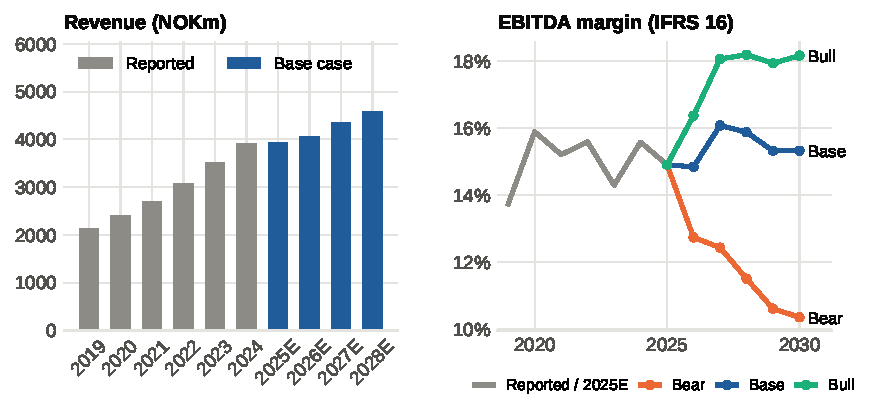
\includegraphics[width=\textwidth]{figures/fig_estimates.pdf}
\vspace{-6pt}
\captionof*{figure}{\footnotesize\color{ink2}Base case revenue and EBITDA margin by scenario. 2026E is flat as price growth matches cost per FTE; 2027E benefits from utilisation recovery and 253 working days against 251.}
\end{center}

\needspace{8\baselineskip}
\subsection{From earnings to cash}
Bouvet's only interest-bearing debt is NOK 353m of IFRS 16 lease liabilities. We treat lease payments as an operating cost, so free cash flow is EBITDA less lease payments, capex and cash tax, plus the cash released by negative working capital as revenue grows. Leases are then not deducted again in the equity bridge. Base case unlevered FCF is NOK 377m in 2026E and NOK 564m in 2035E. EPS is NOK 3.64 in 2025E and NOK 3.77 in 2026E, then rises 18\% to NOK 4.43 in 2027E.

\needspace{12\baselineskip}
\section{Valuation and recommendation}
\needspace{8\baselineskip}
\subsection{Cost of capital}
\begin{center}
\small
\begin{tabularx}{\textwidth}{@{}lrX@{}}
\toprule
\textbf{Component} & \textbf{Value} & \textbf{Basis} \\
\midrule
Risk-free rate & 3.95\% & Norwegian 10-year government bond yield \\
Industry unlevered beta & 0.90 & Western Europe, Computer Services, 210 firms, cash-corrected (Damodaran, 2026b) \\
Lease debt / market cap & 6.2\% & Equity carries the lease leverage because FCF is after lease payments \\
Relevered equity beta & 0.95 & $\beta_L = \beta_U\,(1 + (1-t)\,D/E)$ \\
Market risk premium & 4.23\% & Norway, Aaa, no country risk premium (Damodaran, 2026a) \\
Small-cap premium & 1.0\% & NOK 5.7bn market cap; size premium holds once quality is controlled for (Asness et al., 2018) \\
\textbf{Cost of equity = WACC} & \textbf{9.0\%} & No financial debt \\
\bottomrule
\end{tabularx}
\end{center}
The submission used a raw regression beta of 0.50, most likely measured against a US index. Even after the Blume (1975) adjustment toward 1 that beta is 0.67 and gives a 7.8\% cost of equity, which implies an exit multiple far above where Nordic consultancies trade. We prefer the bottom-up industry beta.

\needspace{8\baselineskip}
\subsection{Discounted cash flow}
Cash flows for 2026E to 2035E are discounted from the 12 February 2026 valuation date with a mid-year convention, and an \texttt{XNPV} on the dated cash flows reproduces the sum exactly. 2035E has only 249 working days, which depresses run-rate FCF because salaries are fixed per FTE, so the terminal base is normalised to the 2026E to 2035E average (NOK 30m).

\begin{center}
\small
\begin{tabularx}{0.75\textwidth}{@{}Xr@{}}
\toprule
\textbf{NOKm} & \textbf{Base} \\
\midrule
PV of FCF 2026E to 2035E & 3,347 \\
PV of terminal value (TGR 2.0\%) & 3,891 \\
Enterprise value & 7,238 \\
Plus cash ex leases, rolled to 31 Dec 2025E & 435 \\
Equity value & 7,673 \\
\textbf{DCF value per share (NOK)} & \textbf{73.9} \\
\midrule
Terminal value share of EV & 54\% \\
Implied exit EV / EBITDA after leases & 11.6x \\
Implied EV / EBIT 2026E (IFRS 16) & 15.1x \\
\bottomrule
\end{tabularx}
\end{center}

\needspace{8\baselineskip}
\subsection{Peer multiples}
Forward earnings multiples price stocks with the smallest error of the common multiples (Liu et al., 2002), so we use 2026E P/E and EV/EBIT. Peer medians are taken with \texttt{AGGREGATE}, which ignores error cells. Bouvet has traded at a 45\% premium to the peer average P/E over 2023 to 2025. That comparison flatters it slightly, because it sets Bouvet's trailing P/E against peers' forward P/E. Its 2024 return on equity of about 83\% against a 2026E peer median of 19\% supports a premium, in line with the warranted-multiple logic of Bhojraj and Lee (2002). Itera is the one peer with similar returns, and it trades at 12x, so we do not pay the full historical premium. We apply 30\%, below the historical level because near-term growth is weaker.

\begin{center}
\small
\begin{tabularx}{\textwidth}{@{}lRRRR@{}}
\toprule
\textbf{2026E} & \textbf{Market cap (NOKm)} & \textbf{P/E} & \textbf{EV/EBIT} & \textbf{EV/EBITDA} \\
\midrule
Itera Asa & 621 & 12.0x & 10.0x & 6.7x \\
Webstep Asa & 533 & 10.0x & 8.9x & 7.1x \\
Know It Ab & 3,826 & 23.1x & 19.1x & 7.6x \\
B3 Consulting Group Ab & 382 & 7.7x & 8.6x & 6.3x \\
Netcompany Group As & 23,946 & 17.0x & 15.4x & 11.6x \\
\midrule
Peer median & 621 & 12.0x & 10.0x & 7.1x \\
\bottomrule
\end{tabularx}
\end{center}
P/E: 12.0x median, 15.6x with the premium, times 2026E EPS of NOK 3.77 gives NOK 58.8. EV/EBIT: 10.0x median, 13.0x with the premium, times 2026E EBIT of NOK 502m, less NIBD including leases, gives NOK 63.0. The average is NOK 60.9 per share. The DCF implies 15.1x 2026E EV/EBIT against a 10.0x peer median, so the premium matters: with no premium at all the target would be NOK 62 and the expected total return +19.8\%, still a BUY.

\needspace{8\baselineskip}
\subsection{Target price and rating}
DCF and multiples get equal weight. Kaplan and Ruback (1995) find DCF at least as accurate as comparables, and blending reduces the error of either method alone. Blended fair value today is NOK 67.4. Rolled forward one year at the cost of equity, less the dividends due over the next 12 months (FY2025 final plus FY2026 interim) of NOK 3.55, this gives NOK 69.9, rounded to a \textbf{target price of NOK 70}. The rating rule is anchored on required return: BUY when the expected total return exceeds the cost of equity by more than 5 percentage points, SELL when it falls short by more than 5.

\begin{center}
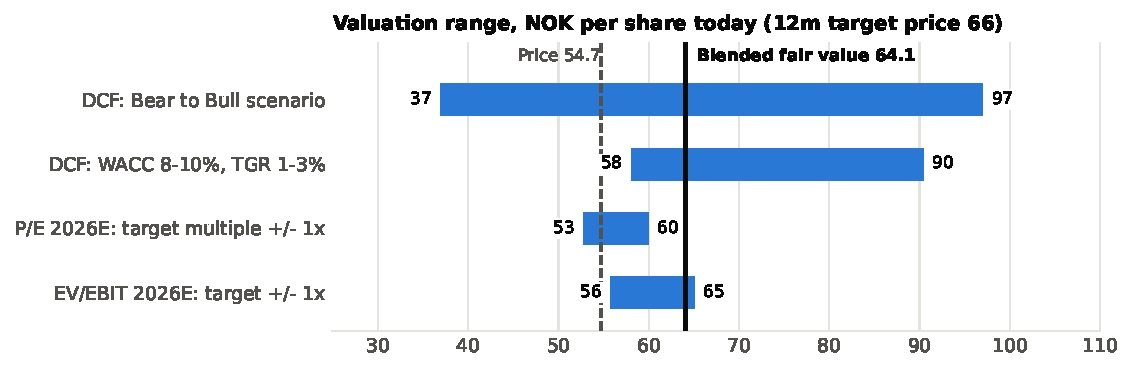
\includegraphics[width=\textwidth]{figures/fig_football.pdf}
\end{center}

\begin{center}
\small
\begin{tabularx}{\textwidth}{@{}lRRRRRr@{}}
\toprule
\textbf{Scenario} & \textbf{DCF} & \textbf{Multiples} & \textbf{Blend today} & \textbf{Target} & \textbf{Total return} & \textbf{Rating} \\
\midrule
Bear & 40.0 & 47.6 & 43.8 & 44 & $-$13.1\% & SELL \\
Base & 73.9 & 60.9 & 67.4 & 70 & +34.5\% & BUY \\
Bull & 101.5 & 70.8 & 86.1 & 90 & +71.0\% & BUY \\
\bottomrule
\end{tabularx}
\end{center}

\begin{minipage}[t]{0.49\textwidth}
\small\textbf{DCF value per share (NOK)}\par
\begin{tabularx}{\linewidth}{@{}lRRRRR@{}}
\toprule
\textbf{WACC} \textbackslash{} \textbf{TGR} & 1.0\% & 1.5\% & 2.0\% & 2.5\% & 3.0\% \\ \midrule
8.0\% & 78.3 & 81.7 & 85.6 & 90.2 & 95.7 \\
8.5\% & 73.3 & 76.1 & 79.3 & 83.1 & 87.5 \\
9.0\% & 68.9 & 71.2 & \textbf{73.9} & 77.0 & 80.6 \\
9.5\% & 65.0 & 67.0 & 69.3 & 71.9 & 74.8 \\
10.0\% & 61.6 & 63.3 & 65.2 & 67.4 & 69.9 \\
\bottomrule
\end{tabularx}
\end{minipage}\hfill
\begin{minipage}[t]{0.49\textwidth}
\small\textbf{12m target price (NOK)}\par
\begin{tabularx}{\linewidth}{@{}lRRRRR@{}}
\toprule
\textbf{Premium} \textbackslash{} \textbf{DCF weight} & 0\% & 25\% & 50\% & 75\% & 100\% \\ \midrule
15.0\% & 55.1 & 60.6 & 66.1 & 71.5 & 77.0 \\
22.5\% & 59.0 & 63.5 & 68.0 & 72.5 & 77.0 \\
30.0\% & 62.8 & 66.3 & \textbf{69.9} & 73.4 & 77.0 \\
37.5\% & 66.6 & 69.2 & 71.8 & 74.4 & 77.0 \\
45.0\% & 70.4 & 72.1 & 73.7 & 75.4 & 77.0 \\
\bottomrule
\end{tabularx}
\end{minipage}

\needspace{12\baselineskip}
\section{Risks and catalysts}
\begin{minipage}[t]{0.49\textwidth}
\textbf{Risks}
\begin{itemize}
\item Utilisation keeps falling through 2026 and Bouvet cuts headcount: the bear case, target NOK 44.
\item The 2026 wage settlement feeds through to cost per FTE faster than price increases.
\item Oil and gas is 42\% of revenue, so a capex pullback by operators hits hard.
\item The top 10 customers are 68\% of revenue.
\item Public sector budgets (18\% of revenue) tighten.
\item Method risk: the valuation rests on the beta choice. A 1pp lower WACC adds NOK 12 per share to the DCF.
\end{itemize}
\end{minipage}\hfill
\begin{minipage}[t]{0.49\textwidth}
\textbf{Catalysts}
\begin{itemize}
\item Q4'25 report: billing ratio and 2026 outlook.
\item Spring 2026 wage settlement against the price increases Bouvet negotiates with clients.
\item The first quarter of positive billing ratio change since Q4'24.
\item 2027 calendar: two more working days than 2026, worth about 0.8\% of revenue at constant rates.
\end{itemize}
\end{minipage}

\needspace{12\baselineskip}
\section{Model integrity and what changed}
\needspace{8\baselineskip}
\subsection{Checks}
The workbook (\texttt{bouvet-case-2026.xlsx}) is built so that it can be audited. Every assumption sits on the Inputs sheet with a source. Colours mark inputs (blue), links (green) and formulas (black), and a Checks sheet must read OK before any number leaves the model. All checks pass in the published version:
\begin{itemize}\small
\item Balance sheet balances, Q3'25 (assets - liabilities and equity) \hfill \textbf{OK}
\item Forecast 2024A revenue ties to Model \hfill \textbf{OK}
\item NETWORKDAYS reproduces reported working days 2021-2024 (sum of abs diff) \hfill \textbf{OK}
\item NETWORKDAYS reproduces reported working days in each of Q1, Q2, Q3 2025 \hfill \textbf{OK}
\item XNPV equals sum of discounted FCF \hfill \textbf{OK}
\item WACC exceeds terminal growth \hfill \textbf{OK}
\item Terminal value share of EV between 50\% and 85\% \hfill \textbf{OK}
\item Sensitivity centre equals DCF value \hfill \textbf{OK}
\item Sensitivity base cell equals unrounded target price \hfill \textbf{OK}
\item Live scenario equals pasted snapshot (target price) \hfill \textbf{OK}
\item Revenue CAGR 2030E-2035E not below TGR \hfill \textbf{OK}
\item No error values in Forecast, DCF, Valuation, WACC, Sensitivity \hfill \textbf{OK}
\item Equity bridge: EV + cash = equity \hfill \textbf{OK}
\end{itemize}

\needspace{8\baselineskip}
\subsection{Changes against the submitted version (12 February 2026)}
\begin{center}
\small
\begin{tabularx}{\textwidth}{@{}lXX@{}}
\toprule
\textbf{Item} & \textbf{Submitted} & \textbf{Revised} \\
\midrule
Rating and target & HOLD, NOK 60.24 & BUY, NOK 70 \\
Cost of capital & 6.06\% on the WACC sheet, 7.30\% hard-coded in the DCF & 9.0\%, one linked value \\
Beta & Raw 0.50 & Bottom-up industry beta relevered to 0.95 \\
Net cash & 251, 513 and 21 used in different places & Cash ex leases 373 at Q3'25, rolled to 435 at year-end (DCF); NIBD incl. leases $-$20.9 (multiples) \\
2024 EBIT in the DCF & 392, a 10\% margin plug & 490 reported \\
Discounting & End of year from 2024 & Mid-year from 12 Feb 2026, \texttt{XNPV} check \\
EPS forecast & 9.7\% of revenue & Driver-based P\&L \\
Target basis & 14x 2027E EPS & Blend of DCF and 2026E multiples, rolled forward 12 months \\
Scenarios & Growth, margin, WACC and TGR moved together (Bull +88\%) & Operating drivers only; WACC fixed \\
Sensitivity and checks & None & Two sensitivity grids, 13 integrity checks \\
\bottomrule
\end{tabularx}
\end{center}

\section*{References}
\small
\begin{list}{}{\leftmargin=12pt \itemindent=-12pt \itemsep=2pt \parsep=0pt}
\item Asness, C., Frazzini, A., Israel, R., Moskowitz, T. J., \& Pedersen, L. H. (2018). Size matters, if you control your junk. \textit{Journal of Financial Economics, 129}(3), 479 to 509. \url{https://doi.org/10.1016/j.jfineco.2018.05.006}
\item Bhojraj, S., \& Lee, C. M. C. (2002). Who is my peer? A valuation-based approach to the selection of comparable firms. \textit{Journal of Accounting Research, 40}(2), 407 to 439. \url{https://doi.org/10.1111/1475-679X.00054}
\item Blume, M. E. (1975). Betas and their regression tendencies. \textit{The Journal of Finance, 30}(3), 785 to 795. \url{https://doi.org/10.1111/j.1540-6261.1975.tb01850.x}
\item Bouvet ASA. (2025). \textit{Quarterly reports Q1 to Q3 2025 and annual report 2024}. \url{https://www.bouvet.no/investor-relations}
\item Damodaran, A. (2025). \textit{Equity risk premiums (ERP): Determinants, estimation, and implications. The 2025 edition}. \url{https://doi.org/10.2139/ssrn.5168609}
\item Damodaran, A. (2026a, January 5). \textit{Country default spreads and risk premiums} [Data set]. \url{https://pages.stern.nyu.edu/~adamodar/New_Home_Page/datafile/ctryprem.html}
\item Damodaran, A. (2026b, January 5). \textit{Betas by sector, Europe} [Data set]. \url{https://pages.stern.nyu.edu/~adamodar/pc/datasets/betaEurope.xls}
\item Kaplan, S. N., \& Ruback, R. S. (1995). The valuation of cash flow forecasts: An empirical analysis. \textit{The Journal of Finance, 50}(4), 1059 to 1093. \url{https://doi.org/10.1111/j.1540-6261.1995.tb04050.x}
\item Liu, J., Nissim, D., \& Thomas, J. (2002). Equity valuation using multiples. \textit{Journal of Accounting Research, 40}(1), 135 to 172. \url{https://doi.org/10.1111/1475-679X.00042}
\end{list}

\vspace{6pt}
{\footnotesize\color{ink2}\textbf{Disclaimer.} This is a student submission to the Pareto Securities Equity Research Case 2026, revised after the competition. It uses only information available on 12 February 2026, is not investment advice and is not affiliated with or endorsed by Pareto Securities or Bouvet ASA. Market sizing figures are as cited in the original case deck and have not been re-verified. Peer multiples are consensus data supplied in the case workbook.}

\end{document}
